\documentclass{beamer}
\usepackage[utf8]{inputenc}
\usepackage{listings}
\usepackage{xcolor}
\usepackage{hyperref}
\usepackage{tikz}
\usetikzlibrary{shapes.geometric, arrows.meta, positioning}

\usetheme{Madrid}
\hypersetup{breaklinks=true}

% Python code style
\definecolor{codegray}{rgb}{0.95,0.95,0.95}
\definecolor{keyword}{rgb}{0.0,0.0,0.6}
\definecolor{comment}{rgb}{0.0,0.5,0.0}
\definecolor{string}{rgb}{0.64,0.08,0.08}

\lstdefinestyle{codeStyle}{
    language=Python,
    backgroundcolor=\color{codegray},
    commentstyle=\color{comment}\itshape,
    keywordstyle=\color{keyword}\bfseries,
    stringstyle=\color{string},
    basicstyle=\ttfamily\footnotesize,
    breaklines=true,
    frame=single,
    showstringspaces=false,
    tabsize=4,
    morekeywords={self, True, False, None, with, as, match, case}
}

% TikZ styles for flowcharts
\tikzset{
    startstop/.style={rectangle, rounded corners, draw, fill=blue!20, minimum width=2cm, minimum height=0.6cm},
    decision/.style={diamond, draw, fill=yellow!20, aspect=2, minimum width=1.5cm},
    process/.style={rectangle, draw, fill=green!10, minimum width=2cm, minimum height=0.6cm},
    arrow/.style={-{Stealth}, thick}
}

\title{Python Programming: Complete Course}
\subtitle{From Basics to Object-Oriented Programming}
\author{Nirajan Bhattarai}
\institute{AI-Driven Development Training}
\date{February 2026}

\begin{document}

% ============================================
% Title Slide
% ============================================
\begin{frame}
    \titlepage
\end{frame}

% ============================================
% Table of Contents
% ============================================
\begin{frame}{Course Outline}
    \tableofcontents
\end{frame}

% ============================================
% SECTION 1: BASICS
% ============================================
\section{Python Basics}

% --------------------------------------------
% LESSON 1: VARIABLES & DATA TYPES
% --------------------------------------------
\begin{frame}{Lesson 1: Variables \& Data Types}
    \small
    \textbf{Concept:} Variables store data in memory.\\[0.5em]
    Python data types: \texttt{int}, \texttt{float}, \texttt{str}, \texttt{bool}, \texttt{NoneType}\\[0.5em]
    \textbf{Type Conversion:} \texttt{int()}, \texttt{float()}, \texttt{str()}, \texttt{bool()}\\[0.5em]
    \textbf{Multiple Use-case Scenarios:}
    \begin{itemize}
        \item Personal Info (name, age, city)
        \item Financial Data (balance, price, quantity)
        \item Sensor Readings (temperature, humidity, status)
    \end{itemize}
\end{frame}

\begin{frame}[fragile]{Lesson 1 Code Example}
    \small
    \begin{lstlisting}[style=codeStyle]
# Personal Info
name, age, city = "Alice", 25, "New York"
is_student = True

# Financial Data
balance, price, quantity = 1500.50, 49.99, 3

# Sensor Readings
temp, humidity, status = 23.5, 65, "OK"

# Type Conversion
age_str = str(age)
price_int = int(price)

# User Input
user_name = input("Enter your name: ")
user_age = int(input("Enter your age: "))
print(f"Hello {user_name}, you are {user_age} years old")
    \end{lstlisting}
\end{frame}

\begin{frame}{Lab 1: Variables}
    \small
    \textbf{Scenario 1: Personal Info}
    \begin{itemize}
        \item Create variables: name, age, city, is\_student
        \item Print info with f-string
        \item Convert age to string and concatenate
        \item Bonus: Check if age $>$ 18 $\to$ ``Adult'', else ``Minor''
    \end{itemize}
    \vspace{0.5em}
    \textbf{Scenario 2: Financial Data}
    \begin{itemize}
        \item Variables: price, quantity, balance
        \item Compute total cost and remaining balance
        \item Bonus: Check if total cost exceeds balance
    \end{itemize}
\end{frame}

% --------------------------------------------
% LESSON 2: OPERATORS
% --------------------------------------------
\begin{frame}{Lesson 2: Operators}
    \small
    \textbf{Arithmetic:} \texttt{+}, \texttt{-}, \texttt{*}, \texttt{/}, \texttt{\%}, \texttt{**}\\[0.5em]
    \textbf{Comparison:} \texttt{>}, \texttt{<}, \texttt{==}, \texttt{!=}, \texttt{>=}, \texttt{<=}\\[0.5em]
    \textbf{Logical:} \texttt{and}, \texttt{or}, \texttt{not}\\[0.5em]
    \textbf{Multiple scenarios:} calculate salary, check pass/fail, logical checks in finance
\end{frame}

\begin{frame}[fragile]{Lesson 2 Code Example}
    \small
    \begin{lstlisting}[style=codeStyle]
# Arithmetic
x, y = 10, 3
print(x+y, x-y, x*y, x/y, x%y, x**y)

# Comparison
print(x > y, x == y, x != y)

# Logical
print(x > 5 and y < 5, x > 5 or y > 5, not(x > y))
    \end{lstlisting}
\end{frame}

\begin{frame}{Lab 2: Operators}
    \small
    \textbf{Scenario 1: Student Grades}
    \begin{itemize}
        \item Scores: math, science, english
        \item Compute total and average
        \item Check if average $>$ 50 $\to$ Pass, else Fail
    \end{itemize}
    \vspace{0.5em}
    \textbf{Scenario 2: Shopping Cart}
    \begin{itemize}
        \item Variables: price, quantity
        \item Total cost, remainder balance
        \item Bonus: Logical check price $>$ 50 or quantity $>$ 5
    \end{itemize}
\end{frame}

% --------------------------------------------
% LESSON 3: STRINGS
% --------------------------------------------
\begin{frame}{Lesson 3: Strings}
    \small
    Strings store text.\\[0.5em]
    \textbf{Methods:} indexing/slicing, \texttt{len()}, \texttt{upper()}, \texttt{lower()}, \texttt{replace()}, \texttt{split()}, \texttt{join()}, \texttt{strip()}\\[0.5em]
    \textbf{Multiple scenarios:} Names, Emails, Product Codes, File Paths
\end{frame}

\begin{frame}[fragile]{Lesson 3 Code Example}
    \small
    \begin{lstlisting}[style=codeStyle]
text = "Python for AI"
print(text.upper(), text.lower(), text.replace("AI", "ML"))
print(text[0:6], text[-2:])

email = "  user@example.com  "
print(email.strip())
    \end{lstlisting}
\end{frame}

\begin{frame}{Lab 3: Strings}
    \small
    \textbf{Scenario 1: Text Processing}
    \begin{itemize}
        \item String: ``Machine Learning''
        \item Print first \& last word
        \item Count vowels
        \item Replace ``Learning'' with ``AI''
        \item Bonus: Reverse string
    \end{itemize}
    \vspace{0.5em}
    \textbf{Scenario 2: File Names}
    \begin{itemize}
        \item Given path: ``/home/user/docs/file.txt''
        \item Extract directory, filename, extension
        \item Convert filename to uppercase
    \end{itemize}
\end{frame}

% --------------------------------------------
% LESSON 4: CONDITIONALS
% --------------------------------------------
\begin{frame}{Lesson 4: Conditional Statements}
    \small
    \texttt{if}/\texttt{elif}/\texttt{else} for branching\\
    \texttt{match-case} (Python 3.10+) for pattern matching
    \vspace{0.5em}
    \begin{center}
        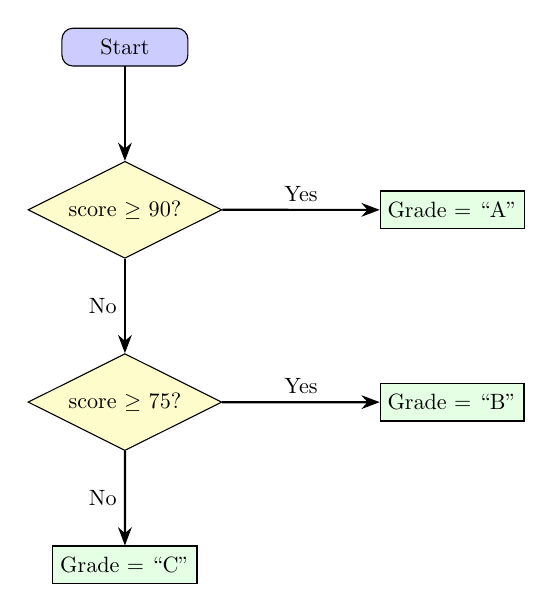
\begin{tikzpicture}[node distance=1.2cm, scale=0.8, every node/.style={scale=0.8}]
            \node (start) [startstop] {Start};
            \node (cond1) [decision, below=of start] {score $\geq$ 90?};
            \node (gradeA) [process, right=2cm of cond1] {Grade = ``A''};
            \node (cond2) [decision, below=of cond1] {score $\geq$ 75?};
            \node (gradeB) [process, right=2cm of cond2] {Grade = ``B''};
            \node (gradeC) [process, below=of cond2] {Grade = ``C''};
            
            \draw[arrow] (start) -- (cond1);
            \draw[arrow] (cond1) -- node[above] {Yes} (gradeA);
            \draw[arrow] (cond1) -- node[left] {No} (cond2);
            \draw[arrow] (cond2) -- node[above] {Yes} (gradeB);
            \draw[arrow] (cond2) -- node[left] {No} (gradeC);
        \end{tikzpicture}
    \end{center}
\end{frame}

\begin{frame}[fragile]{Lesson 4 Code Example (if/else)}
    \small
    \begin{lstlisting}[style=codeStyle]
# Simple if/else
age = 20
if age >= 18:
    print("Adult")
else:
    print("Minor")

# if/elif/else chain
score = 85
if score >= 90:
    grade = "A"
elif score >= 75:
    grade = "B"
elif score >= 60:
    grade = "C"
else:
    grade = "F"
print(f"Grade: {grade}")
    \end{lstlisting}
\end{frame}

\begin{frame}[fragile]{Lesson 4 Code Example (match-case)}
    \small
    \begin{lstlisting}[style=codeStyle]
# match-case (Python 3.10+)
fruit = "apple"
match fruit:
    case "apple":
        print("Red fruit")
    case "banana":
        print("Yellow fruit")
    case _:
        print("Unknown fruit")

# Nested conditionals
x, y = 10, 5
if x > 0:
    if y > 0:
        print("Both positive")
    else:
        print("x positive, y non-positive")
    \end{lstlisting}
\end{frame}

\begin{frame}{Lab 4: Conditionals}
    \small
    \textbf{Scenario 1: Bank Balance}
    \begin{itemize}
        \item balance $>$ 0 $\to$ Positive, $=$ 0 $\to$ Zero, $<$ 0 $\to$ Overdraft
        \item Bonus: match-case ranges: low, medium, high
    \end{itemize}
    \vspace{0.5em}
    \textbf{Scenario 2: Ticket Pricing}
    \begin{itemize}
        \item age $<$ 12 $\to$ child, 12--59 $\to$ adult, 60+ $\to$ senior
        \item Bonus: extra discount for VIP
    \end{itemize}
    \vspace{0.5em}
    \textbf{Scenario 3: Login System}
    \begin{itemize}
        \item Check username and password match
        \item Nested if: check if account is active
        \item Bonus: limit login attempts to 3
    \end{itemize}
\end{frame}

% --------------------------------------------
% LESSON 5: LOOPS
% --------------------------------------------
\begin{frame}{Lesson 5: Loops}
    \small
    \texttt{for} loop: iterate sequences/range\\
    \texttt{while} loop: repeat until condition False\\
    \texttt{break}/\texttt{continue}: control loop flow
    \vspace{0.5em}
    \begin{center}
        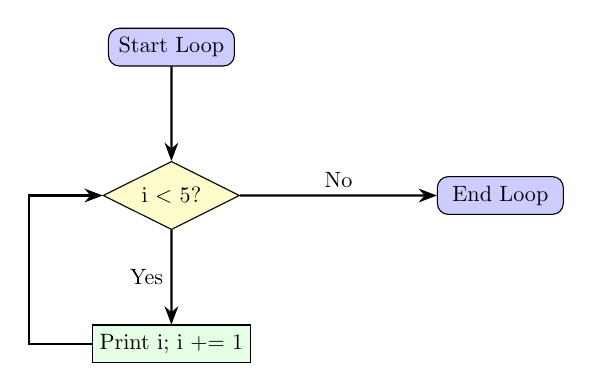
\begin{tikzpicture}[node distance=1.2cm, scale=0.8, every node/.style={scale=0.8}]
            \node (start) [startstop] {Start Loop};
            \node (cond) [decision, below=of start] {i $<$ 5?};
            \node (body) [process, below=of cond] {Print i; i += 1};
            \node (end) [startstop, right=2.5cm of cond] {End Loop};
            
            \draw[arrow] (start) -- (cond);
            \draw[arrow] (cond) -- node[above] {No} (end);
            \draw[arrow] (cond) -- node[left] {Yes} (body);
            \draw[arrow] (body.west) -- ++(-1,0) |- (cond.west);
        \end{tikzpicture}
    \end{center}
\end{frame}

\begin{frame}[fragile]{Lesson 5 Code Example}
    \small
    \begin{lstlisting}[style=codeStyle]
# for loop with range
for i in range(5):
    print(i)

# for loop with list
fruits = ["apple", "banana", "cherry"]
for fruit in fruits:
    print(fruit)

# while loop
x = 0
while x < 3:
    print(x)
    x += 1

# break and continue
for i in range(10):
    if i == 3:
        continue  # skip 3
    if i == 7:
        break     # stop at 7
    print(i)
    \end{lstlisting}
\end{frame}

\begin{frame}{Lab 5: Loops}
    \small
    \textbf{Scenario 1: Multiples of 3}
    \begin{itemize}
        \item Print multiples of 3 from 1--20
        \item Store in list
        \item Bonus: list comprehension
    \end{itemize}
    \vspace{0.5em}
    \textbf{Scenario 2: Nested Loop Matrix}
    \begin{itemize}
        \item Given matrix, print all elements
        \item Create flat list using nested comprehension
        \item Bonus: filter even numbers
    \end{itemize}
\end{frame}

% --------------------------------------------
% LESSON 6: FUNCTIONS
% --------------------------------------------
\begin{frame}{Lesson 6: Functions}
    \small
    \texttt{def name(params):} define function\\
    \texttt{return} for return value\\
    Default arguments, *args, **kwargs
    \vspace{0.5em}
    \begin{center}
        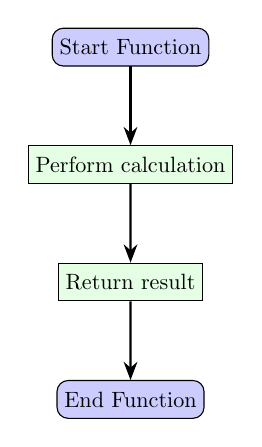
\begin{tikzpicture}[node distance=1cm, scale=0.8, every node/.style={scale=0.8}]
            \node (start) [startstop] {Start Function};
            \node (process) [process, below=of start] {Perform calculation};
            \node (return) [process, below=of process] {Return result};
            \node (end) [startstop, below=of return] {End Function};
            
            \draw[arrow] (start) -- (process);
            \draw[arrow] (process) -- (return);
            \draw[arrow] (return) -- (end);
        \end{tikzpicture}
    \end{center}
\end{frame}

\begin{frame}[fragile]{Lesson 6 Code Example}
    \small
    \begin{lstlisting}[style=codeStyle]
# Basic function with default argument
def greet(name="Alice"):
    return f"Hello, {name}!"

# Function with multiple returns
def divide(a, b):
    if b == 0:
        return None, "Error: Division by zero"
    return a / b, "Success"

# *args - variable positional arguments
def sum_all(*args):
    return sum(args)

# **kwargs - variable keyword arguments
def print_info(**kwargs):
    for key, value in kwargs.items():
        print(f"{key}: {value}")

print(sum_all(1, 2, 3, 4, 5))  # 15
print_info(name="Alice", age=25, city="NYC")
    \end{lstlisting}
\end{frame}

\begin{frame}{Lab 6: Functions}
    \small
    \textbf{Scenario 1: Calculator}
    \begin{itemize}
        \item Function: product of two numbers
        \item Function: factorial
        \item Bonus: sum list
    \end{itemize}
    \vspace{0.5em}
    \textbf{Scenario 2: Temperature Conversion}
    \begin{itemize}
        \item Celsius to Fahrenheit
        \item Fahrenheit to Celsius
        \item Bonus: average conversion for a list of temps
    \end{itemize}
\end{frame}

% --------------------------------------------
% LESSON 6B: ERROR HANDLING
% --------------------------------------------
\begin{frame}{Lesson 6B: Error Handling (try/except)}
    \small
    \textbf{Concept:} Handle runtime errors gracefully\\[0.5em]
    \textbf{Keywords:} \texttt{try}, \texttt{except}, \texttt{else}, \texttt{finally}, \texttt{raise}\\[0.5em]
    \textbf{Common Exceptions:}
    \begin{itemize}
        \item \texttt{ValueError} -- invalid value conversion
        \item \texttt{TypeError} -- wrong type operation
        \item \texttt{ZeroDivisionError} -- division by zero
        \item \texttt{FileNotFoundError} -- file doesn't exist
        \item \texttt{KeyError} -- dict key not found
        \item \texttt{IndexError} -- list index out of range
    \end{itemize}
\end{frame}

\begin{frame}[fragile]{Lesson 6B Code Example}
    \small
    \begin{lstlisting}[style=codeStyle]
# Basic try/except
try:
    num = int(input("Enter number: "))
    result = 10 / num
except ValueError:
    print("Invalid input!")
except ZeroDivisionError:
    print("Cannot divide by zero!")
else:
    print(f"Result: {result}")
finally:
    print("Execution complete")

# Raising exceptions
def divide(a, b):
    if b == 0:
        raise ValueError("Divisor cannot be zero")
    return a / b
    \end{lstlisting}
\end{frame}

\begin{frame}{Lab 6B: Error Handling}
    \small
    \textbf{Scenario 1: Safe Calculator}
    \begin{itemize}
        \item Create divide function with try/except
        \item Handle ZeroDivisionError and TypeError
        \item Bonus: Log errors to a file
    \end{itemize}
    \vspace{0.5em}
    \textbf{Scenario 2: File Reader}
    \begin{itemize}
        \item Try to open and read a file
        \item Handle FileNotFoundError
        \item Use finally to ensure cleanup
        \item Bonus: Retry mechanism for failed reads
    \end{itemize}
\end{frame}

% ============================================
% SECTION 2: COLLECTIONS AND ADVANCED CONCEPTS
% ============================================
\section{Collections and Advanced Python Concepts}

% --------------------------------------------
% LESSON 7: LISTS
% --------------------------------------------
\begin{frame}{Lesson 7: Python Lists -- Basics}
    \small
    Lists store ordered sequences.\\[0.5em]
    \textbf{Methods:} \texttt{append}, \texttt{extend}, \texttt{insert}, \texttt{remove}, \texttt{pop}, \texttt{clear}, \texttt{index}, \texttt{count}, \texttt{copy}\\[0.5em]
    \textbf{Scenario Examples:} fruits, numbers, tasks, sensor readings
\end{frame}

\begin{frame}[fragile]{Lesson 7 Code Example}
    \small
    \begin{lstlisting}[style=codeStyle]
fruits = ["apple", "banana", "cherry"]
fruits.append("orange")
fruits.insert(1, "mango")
fruits.remove("banana")
print(fruits[0], fruits[-1])
    \end{lstlisting}
\end{frame}

\begin{frame}{Lab 7: Lists}
    \small
    \textbf{Scenario 1: Grocery List}
    \begin{itemize}
        \item Add 3 items, remove 1, print first \& last
        \item Bonus: Sort alphabetically, reverse order
    \end{itemize}
    \vspace{0.5em}
    \textbf{Scenario 2: Numbers}
    \begin{itemize}
        \item List of 1--10, filter even numbers using loop
        \item Bonus: Use list comprehension
    \end{itemize}
\end{frame}

% --------------------------------------------
% LESSON 7B: TUPLES & SETS
% --------------------------------------------
\begin{frame}{Lesson 7B: Tuples \& Sets}
    \small
    \textbf{Tuples:} Immutable ordered sequences\\[0.3em]
    \begin{itemize}
        \item Created with \texttt{()} or \texttt{tuple()}
        \item Cannot modify after creation
        \item Use for fixed data (coordinates, RGB colors)
    \end{itemize}
    \vspace{0.5em}
    \textbf{Sets:} Unordered collection of unique elements\\[0.3em]
    \begin{itemize}
        \item Created with \texttt{\{\}} or \texttt{set()}
        \item No duplicates allowed
        \item Fast membership testing
        \item Set operations: union, intersection, difference
    \end{itemize}
\end{frame}

\begin{frame}[fragile]{Lesson 7B Code Example}
    \small
    \begin{lstlisting}[style=codeStyle]
# Tuples - immutable
point = (10, 20)
x, y = point  # unpacking
colors = ("red", "green", "blue")
print(colors[0], len(colors))

# Sets - unique elements only
numbers = {1, 2, 3, 3, 2, 1}  # {1, 2, 3}
numbers.add(4)
numbers.remove(1)

# Set operations
a = {1, 2, 3, 4}
b = {3, 4, 5, 6}
print(a | b)  # union: {1, 2, 3, 4, 5, 6}
print(a & b)  # intersection: {3, 4}
print(a - b)  # difference: {1, 2}
print(3 in a) # membership: True
    \end{lstlisting}
\end{frame}

\begin{frame}{Lab 7B: Tuples \& Sets}
    \small
    \textbf{Scenario 1: Coordinate System}
    \begin{itemize}
        \item Create tuple for 2D point (x, y)
        \item Unpack and calculate distance from origin
        \item Bonus: List of points, find furthest from origin
    \end{itemize}
    \vspace{0.5em}
    \textbf{Scenario 2: Unique Items}
    \begin{itemize}
        \item Given list with duplicates, get unique items using set
        \item Find common items between two lists
        \item Bonus: Remove items that appear in both lists
    \end{itemize}
\end{frame}

% --------------------------------------------
% LESSON 8: ADVANCED LISTS
% --------------------------------------------
\begin{frame}{Lesson 8: List Comprehensions \& Map/Filter}
    \small
    \textbf{Concepts:} Transform, filter, map, lambda functions
    \vspace{0.5em}
    \begin{center}
        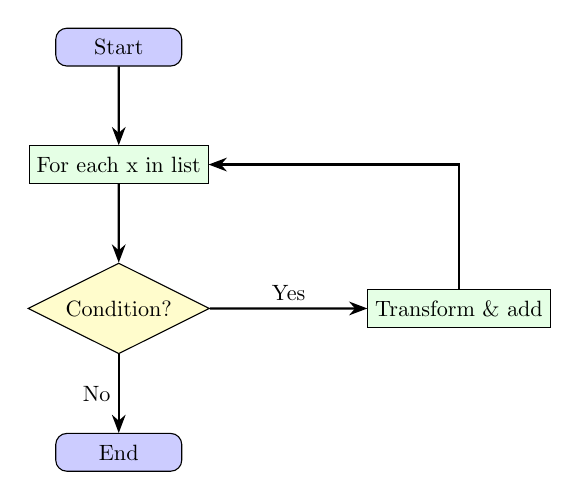
\begin{tikzpicture}[node distance=1cm, scale=0.8, every node/.style={scale=0.8}]
            \node (start) [startstop] {Start};
            \node (loop) [process, below=of start] {For each x in list};
            \node (cond) [decision, below=of loop] {Condition?};
            \node (action) [process, right=2cm of cond] {Transform \& add};
            \node (end) [startstop, below=of cond] {End};
            
            \draw[arrow] (start) -- (loop);
            \draw[arrow] (loop) -- (cond);
            \draw[arrow] (cond) -- node[above] {Yes} (action);
            \draw[arrow] (cond) -- node[left] {No} (end);
            \draw[arrow] (action) |- (loop);
        \end{tikzpicture}
    \end{center}
\end{frame}

\begin{frame}[fragile]{Lesson 8 Code Example}
    \small
    \begin{lstlisting}[style=codeStyle]
lst = [1, 2, 3, 4, 5]

# List comprehension: square even numbers
squared = [x**2 for x in lst if x % 2 == 0]

# Lambda + map: double numbers
doubled = list(map(lambda x: x * 2, lst))

# Filter: numbers > 3
filtered = list(filter(lambda x: x > 3, lst))

print(squared, doubled, filtered)
    \end{lstlisting}
\end{frame}

\begin{frame}{Lab 8: Advanced Lists}
    \small
    \textbf{Scenario 1: Student Scores}
    \begin{itemize}
        \item Scores = [78, 85, 62, 90, 55]
        \item Filter scores $>$ 70, square them, sum total
        \item Bonus: use lambda + map + filter
    \end{itemize}
    \vspace{0.5em}
    \textbf{Scenario 2: Product Prices}
    \begin{itemize}
        \item Prices = [10, 25, 50, 5, 40]
        \item Apply discount 10\% to all, keep only discounted $>$ 20
        \item Bonus: nested list comprehension with tax
    \end{itemize}
\end{frame}

% --------------------------------------------
% LESSON 8B: LAMBDA & SCOPE
% --------------------------------------------
\begin{frame}{Lesson 8B: Lambda Functions \& Variable Scope}
    \small
    \textbf{Lambda:} Anonymous single-expression functions\\[0.3em]
    \texttt{lambda args: expression}\\[0.5em]
    \textbf{Variable Scope:}
    \begin{itemize}
        \item \textbf{Local} -- inside function
        \item \textbf{Enclosing} -- outer function (nested)
        \item \textbf{Global} -- module level
        \item \textbf{Built-in} -- Python built-ins
    \end{itemize}
    \vspace{0.3em}
    Use \texttt{global} keyword to modify global variables\\
    Use \texttt{nonlocal} for enclosing scope
\end{frame}

\begin{frame}[fragile]{Lesson 8B Code Example}
    \small
    \begin{lstlisting}[style=codeStyle]
# Lambda functions
square = lambda x: x ** 2
add = lambda a, b: a + b
print(square(5), add(3, 4))

# Sorting with lambda
students = [("Alice", 85), ("Bob", 92), ("Eve", 78)]
students.sort(key=lambda x: x[1], reverse=True)

# Variable scope
count = 0  # global

def increment():
    global count
    count += 1

def outer():
    x = 10
    def inner():
        nonlocal x
        x += 5
    inner()
    return x  # 15
    \end{lstlisting}
\end{frame}

\begin{frame}{Lab 8B: Lambda \& Scope}
    \small
    \textbf{Scenario 1: Sorting}
    \begin{itemize}
        \item Sort list of dicts by specific key using lambda
        \item Sort strings by length
        \item Bonus: Sort by multiple criteria
    \end{itemize}
    \vspace{0.5em}
    \textbf{Scenario 2: Counter}
    \begin{itemize}
        \item Create counter using global variable
        \item Create counter using closure (nested function)
        \item Bonus: Compare both approaches
    \end{itemize}
\end{frame}

% --------------------------------------------
% LESSON 9: DICTIONARIES
% --------------------------------------------
\begin{frame}{Lesson 9: Dictionaries}
    \small
    Key-value storage, unordered, mutable.\\[0.5em]
    \textbf{Methods:} \texttt{keys()}, \texttt{values()}, \texttt{items()}, \texttt{get()}, \texttt{update()}, \texttt{pop()}, \texttt{popitem()}, \texttt{clear}\\[0.5em]
    \textbf{Scenarios:} Student grades, product info, employee records
\end{frame}

\begin{frame}[fragile]{Lesson 9 Code Example}
    \small
    \begin{lstlisting}[style=codeStyle]
grades = {"Alice": [85, 90], "Bob": [78, 88]}

# Add new student
grades["Charlie"] = [92, 95]

# Average per student (dict comprehension)
avg = {k: sum(v)/len(v) for k, v in grades.items()}

# Map + lambda for scores
squared = {k: list(map(lambda x: x**2, v)) 
           for k, v in grades.items()}

print(avg, squared)
    \end{lstlisting}
\end{frame}

\begin{frame}{Lab 9: Dictionaries}
    \small
    \textbf{Scenario 1: Employee Records}
    \begin{itemize}
        \item Create dict: \texttt{\{"John": [25, "HR"], "Alice": [30, "IT"]\}}
        \item Add new employee, update department
        \item Bonus: filter age $>$ 28
    \end{itemize}
    \vspace{0.5em}
    \textbf{Scenario 2: Grades}
    \begin{itemize}
        \item Compute average score per student
        \item Identify top students avg $>$ 85
        \item Bonus: write top students to file
    \end{itemize}
\end{frame}

% --------------------------------------------
% LESSON 10: FILE HANDLING
% --------------------------------------------
\begin{frame}{Lesson 10: File Handling}
    \small
    Read/write text files.\\[0.5em]
    \textbf{Methods:} \texttt{open()}, \texttt{read()}, \texttt{readline()}, \texttt{readlines()}, \texttt{write()}, \texttt{writelines()}, \texttt{close()}\\[0.5em]
    Use \texttt{with} for automatic closing
    \vspace{0.5em}
    \begin{center}
        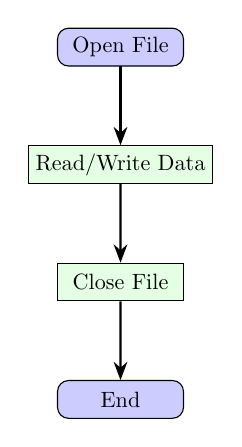
\begin{tikzpicture}[node distance=1cm, scale=0.8, every node/.style={scale=0.8}]
            \node (start) [startstop] {Open File};
            \node (read) [process, below=of start] {Read/Write Data};
            \node (close) [process, below=of read] {Close File};
            \node (end) [startstop, below=of close] {End};
            
            \draw[arrow] (start) -- (read);
            \draw[arrow] (read) -- (close);
            \draw[arrow] (close) -- (end);
        \end{tikzpicture}
    \end{center}
\end{frame}

\begin{frame}[fragile]{Lesson 10 Code Example}
    \small
    \begin{lstlisting}[style=codeStyle]
# Write to file
with open("data.txt", "w") as f:
    f.write("Hello Python\n")
    f.write("Line 2\n")

# Read file
with open("data.txt", "r") as f:
    for line in f:
        print(line.strip())
    \end{lstlisting}
\end{frame}

\begin{frame}{Lab 10: File Handling}
    \small
    \textbf{Scenario 1: Log File}
    \begin{itemize}
        \item Write 5 log entries to ``log.txt''
        \item Read file and print only lines containing ``error''
        \item Bonus: Count error lines
    \end{itemize}
    \vspace{0.5em}
    \textbf{Scenario 2: Student Scores}
    \begin{itemize}
        \item Write student grades to ``grades.txt''
        \item Read and compute average score per student
        \item Bonus: Filter students avg $>$ 80
    \end{itemize}
\end{frame}

% --------------------------------------------
% LESSON 11: NUMPY ARRAYS
% --------------------------------------------
\begin{frame}{Lesson 11: NumPy Arrays}
    \small
    NumPy arrays for efficient numerical computation\\[0.5em]
    \textbf{Key Data Structures:}
    \begin{itemize}
        \item \texttt{ndarray} -- N-dimensional array (homogeneous data)
        \item Supports 1D (vector), 2D (matrix), nD (tensor)
    \end{itemize}
    \vspace{0.3em}
    \textbf{Array Creation:}
    \begin{itemize}
        \item \texttt{np.array()} -- from list/tuple
        \item \texttt{np.zeros()}, \texttt{np.ones()} -- filled arrays
        \item \texttt{np.arange()}, \texttt{np.linspace()} -- sequences
        \item \texttt{np.random.rand()} -- random arrays
    \end{itemize}
\end{frame}

\begin{frame}{Lesson 11: NumPy Properties \& Operations}
    \small
    \textbf{Array Properties:}
    \begin{itemize}
        \item \texttt{shape} -- dimensions (rows, cols)
        \item \texttt{dtype} -- data type (int64, float64)
        \item \texttt{ndim} -- number of dimensions
        \item \texttt{size} -- total elements
    \end{itemize}
    \vspace{0.3em}
    \textbf{Key Operations:}
    \begin{itemize}
        \item Element-wise: \texttt{+}, \texttt{-}, \texttt{*}, \texttt{/}, \texttt{**}
        \item Aggregation: \texttt{sum()}, \texttt{mean()}, \texttt{std()}, \texttt{min()}, \texttt{max()}
        \item Reshaping: \texttt{reshape()}, \texttt{flatten()}, \texttt{transpose()}
        \item Indexing: slicing, boolean masks, fancy indexing
    \end{itemize}
\end{frame}

\begin{frame}[fragile]{Lesson 11 Code Example}
    \small
    \begin{lstlisting}[style=codeStyle]
import numpy as np

# Array creation
arr = np.array([[1, 2, 3], [4, 5, 6], [7, 8, 9]])
zeros = np.zeros((2, 3))      # 2x3 array of zeros
ones = np.ones((3, 3))        # 3x3 array of ones
seq = np.arange(0, 10, 2)     # [0, 2, 4, 6, 8]

# Properties
print(arr.shape, arr.dtype, arr.ndim)

# Operations
print(arr * 2)                # element-wise multiply
print(arr.sum(axis=0))        # sum per column
print(arr.mean(axis=1))       # mean per row

# Boolean indexing
mask = arr > 5
print(arr[mask])              # [6, 7, 8, 9]
    \end{lstlisting}
\end{frame}

\begin{frame}{Lab 11: NumPy Arrays}
    \small
    \textbf{Scenario 1: Matrix Operations}
    \begin{itemize}
        \item Create 3x3 matrix using \texttt{np.array()}
        \item Flatten and filter elements $>$ 5
        \item Compute sum, mean, std deviation
        \item Bonus: Transpose and matrix multiply with \texttt{@}
    \end{itemize}
    \vspace{0.5em}
    \textbf{Scenario 2: Sensor Data}
    \begin{itemize}
        \item Create 1D array of 100 random readings
        \item Compute max, min, average
        \item Use boolean mask for readings $>$ threshold
        \item Bonus: Reshape to 10x10 and compute row means
    \end{itemize}
\end{frame}

% --------------------------------------------
% LESSON 11B: PANDAS DATA STRUCTURES
% --------------------------------------------
\begin{frame}{Lesson 11B: Pandas Data Structures}
    \small
    Pandas provides powerful data structures for data analysis\\[0.5em]
    \textbf{Key Data Structures:}
    \begin{itemize}
        \item \texttt{Series} -- 1D labeled array (like a column)
        \item \texttt{DataFrame} -- 2D labeled table (rows \& columns)
    \end{itemize}
    \vspace{0.3em}
    \textbf{Why Pandas?}
    \begin{itemize}
        \item Handles heterogeneous data (mixed types)
        \item Built-in handling of missing values (NaN)
        \item Powerful indexing and filtering
        \item Easy file I/O (CSV, Excel, JSON, SQL)
    \end{itemize}
\end{frame}

\begin{frame}{Lesson 11B: Series \& DataFrame}
    \small
    \textbf{Series:} 1D array with labels (index)
    \begin{itemize}
        \item Created from list, dict, or scalar
        \item Access by label: \texttt{s['a']} or position: \texttt{s[0]}
    \end{itemize}
    \vspace{0.5em}
    \textbf{DataFrame:} 2D table with row/column labels
    \begin{itemize}
        \item Created from dict, list of dicts, or 2D array
        \item Columns = Series
        \item Access column: \texttt{df['col']} or \texttt{df.col}
        \item Access row: \texttt{df.loc['label']} or \texttt{df.iloc[0]}
    \end{itemize}
\end{frame}

\begin{frame}[fragile]{Lesson 11B Code Example (Creation)}
    \small
    \begin{lstlisting}[style=codeStyle]
import pandas as pd

# Series - 1D labeled array
s = pd.Series([10, 20, 30], index=['a', 'b', 'c'])
print(s['b'])  # 20

# DataFrame from dict
df = pd.DataFrame({
    'Name': ['Alice', 'Bob', 'Charlie'],
    'Age': [25, 30, 35],
    'City': ['NYC', 'LA', 'Chicago']
})
print(df)

# DataFrame from list of dicts
data = [{'x': 1, 'y': 2}, {'x': 3, 'y': 4}]
df2 = pd.DataFrame(data)
    \end{lstlisting}
\end{frame}

\begin{frame}[fragile]{Lesson 11B Code Example (Operations)}
    \small
    \begin{lstlisting}[style=codeStyle]
import pandas as pd

df = pd.DataFrame({
    'Name': ['Alice', 'Bob', 'Charlie', 'Diana'],
    'Score': [85, 92, 78, 95],
    'Department': ['HR', 'IT', 'IT', 'HR']
})

# Basic properties
print(df.shape, df.columns, df.dtypes)

# Selection
print(df['Name'])           # single column
print(df[['Name', 'Score']])# multiple columns
print(df.loc[0])            # row by label
print(df.iloc[0:2])         # rows by position

# Filtering
high_scores = df[df['Score'] > 80]
it_dept = df[df['Department'] == 'IT']
    \end{lstlisting}
\end{frame}

\begin{frame}[fragile]{Lesson 11B Code Example (Analysis)}
    \small
    \begin{lstlisting}[style=codeStyle]
# Aggregation
print(df['Score'].mean())    # average score
print(df['Score'].max())     # max score
print(df.describe())         # summary statistics

# GroupBy - split-apply-combine
grouped = df.groupby('Department')['Score'].mean()
print(grouped)

# Adding/modifying columns
df['Passed'] = df['Score'] > 80
df['Bonus'] = df['Score'] * 0.1

# Sorting
df_sorted = df.sort_values('Score', ascending=False)

# Missing data
df['Grade'] = [None, 'A', 'B', None]
df['Grade'].fillna('C', inplace=True)
    \end{lstlisting}
\end{frame}

\begin{frame}[fragile]{Lesson 11B Code Example (File I/O)}
    \small
    \begin{lstlisting}[style=codeStyle]
import pandas as pd

# Read from CSV
df = pd.read_csv('data.csv')

# Write to CSV
df.to_csv('output.csv', index=False)

# Read from Excel
df = pd.read_excel('data.xlsx', sheet_name='Sheet1')

# Read from JSON
df = pd.read_json('data.json')

# Quick data exploration
print(df.head())       # first 5 rows
print(df.tail())       # last 5 rows
print(df.info())       # column types & non-null counts
print(df.describe())   # statistical summary
    \end{lstlisting}
\end{frame}

\begin{frame}{Lab 11B: Pandas Data Structures}
    \small
    \textbf{Scenario 1: Employee Database}
    \begin{itemize}
        \item Create DataFrame with: Name, Age, Dept, Salary
        \item Filter employees with salary $>$ 50000
        \item Group by department, compute average salary
        \item Bonus: Add ``Bonus'' column (10\% of salary)
    \end{itemize}
    \vspace{0.5em}
    \textbf{Scenario 2: Sales Analysis}
    \begin{itemize}
        \item Create DataFrame: Product, Quantity, Price, Date
        \item Calculate total revenue (Quantity $\times$ Price)
        \item Find top 3 products by revenue
        \item Bonus: Read from CSV, group by date, plot trends
    \end{itemize}
\end{frame}

% --------------------------------------------
% LESSON 12: JSON & REGEX
% --------------------------------------------
\begin{frame}{Lesson 12: JSON \& Regex}
    \small
    \textbf{JSON:} exchange data between systems\\
    \texttt{json.loads()}, \texttt{json.dumps()}\\[0.5em]
    \textbf{Regex:} pattern matching, validation\\
    \texttt{re.search()}, \texttt{re.findall()}, \texttt{re.sub()}
\end{frame}

\begin{frame}[fragile]{Lesson 12 Code Example}
    \small
    \begin{lstlisting}[style=codeStyle]
import json
import re

# JSON
data = '{"name": "Alice", "age": 25}'
parsed = json.loads(data)
print(parsed["name"])

# Regex
text = "Email: user@example.com"
match = re.search(r"\S+@\S+", text)
if match:
    print(match.group())
    \end{lstlisting}
\end{frame}

\begin{frame}{Lab 12: JSON \& Regex}
    \small
    \textbf{Scenario 1: Student JSON}
    \begin{itemize}
        \item Parse JSON string of students with scores
        \item Compute average per student
        \item Bonus: Filter students avg $>$ 80
    \end{itemize}
    \vspace{0.5em}
    \textbf{Scenario 2: Email Validation}
    \begin{itemize}
        \item Given a list of emails, find valid ones using regex
        \item Bonus: Replace domain from old to new
    \end{itemize}
\end{frame}

% ============================================
% SECTION 3: ADDITIONAL TOPICS
% ============================================
\section{Additional Topics}

% --------------------------------------------
% LESSON 13: MODULES & PACKAGES
% --------------------------------------------
\begin{frame}{Lesson 13: Modules \& Packages}
    \small
    \textbf{Module:} Single Python file with reusable code\\[0.3em]
    \textbf{Package:} Directory containing multiple modules\\[0.5em]
    \textbf{Import Styles:}
    \begin{itemize}
        \item \texttt{import module}
        \item \texttt{from module import function}
        \item \texttt{from module import *}
        \item \texttt{import module as alias}
    \end{itemize}
    \vspace{0.3em}
    \textbf{Creating Modules:} Any \texttt{.py} file is a module\\
    \textbf{\_\_name\_\_:} Use \texttt{if \_\_name\_\_ == "\_\_main\_\_":}
\end{frame}

\begin{frame}[fragile]{Lesson 13 Code Example}
    \small
    \begin{lstlisting}[style=codeStyle]
# Using standard library modules
import math
import random
import datetime

print(math.sqrt(16))
print(random.randint(1, 100))
print(datetime.datetime.now())

# Creating your own module (mymodule.py)
# def greet(name):
#     return f"Hello, {name}!"

# Using your module
# from mymodule import greet
# print(greet("Alice"))

# Main guard
if __name__ == "__main__":
    # This runs only when file is executed directly
    print("Running as main program")
    \end{lstlisting}
\end{frame}

\begin{frame}{Lab 13: Modules \& Packages}
    \small
    \textbf{Scenario 1: Utility Module}
    \begin{itemize}
        \item Create module with math helper functions
        \item Import and use in another file
        \item Bonus: Add documentation strings
    \end{itemize}
    \vspace{0.5em}
    \textbf{Scenario 2: Standard Library}
    \begin{itemize}
        \item Use \texttt{os} module for file operations
        \item Use \texttt{datetime} for date calculations
        \item Bonus: Explore \texttt{collections} module
    \end{itemize}
\end{frame}

% ============================================
% SUMMARY & CLOSING
% ============================================
\section{Summary}

\begin{frame}{Course Summary}
    \small
    \textbf{Section 1: Python Basics (Lessons 1--6B)}
    \begin{itemize}
        \item Variables, Data Types, Input/Output
        \item Operators, Strings
        \item Conditionals (if/elif/else, match-case)
        \item Loops (for, while, break, continue)
        \item Functions (*args, **kwargs), Error Handling
    \end{itemize}
    \vspace{0.5em}
    \textbf{Section 2: Collections \& Data (Lessons 7--12)}
    \begin{itemize}
        \item Lists, Tuples, Sets, Dictionaries
        \item List Comprehensions, Lambda, Map/Filter
        \item File Handling, JSON, Regex
        \item NumPy Arrays (ndarray, operations, indexing)
        \item Pandas (Series, DataFrame, GroupBy, I/O)
    \end{itemize}
    \vspace{0.5em}
    \textbf{Section 3: Additional Topics (Lesson 13)}
    \begin{itemize}
        \item Modules \& Packages
    \end{itemize}
\end{frame}

\begin{frame}{Next Steps}
    \small
    \textbf{Practice Resources:}
    \begin{itemize}
        \item Complete all lab exercises
        \item Build mini-projects combining concepts
        \item Explore Python documentation
    \end{itemize}
    \vspace{0.5em}
    \textbf{Topics to Explore Next:}
    \begin{itemize}
        \item Object-Oriented Programming (Classes)
        \item Decorators \& Generators
        \item Testing (pytest, unittest)
        \item Virtual Environments (venv, pip)
        \item Web frameworks (Flask, Django, FastAPI)
        \item Data Science (Pandas, Matplotlib)
    \end{itemize}
    \vspace{1em}
    \centering
    \textbf{\Large Questions?}
\end{frame}

\end{document}